
%% see http://latex-beamer.sourceforge.net/
%% idea contributed by H. Turgut Uyar
%% template based on a template by Till Tantau
%% this template is still evolving - it might differ in future releases!

\documentclass[xcolor={usenames,dvipsnames}]{beamer}
\usepackage{booktabs}


% THEME
% =========================================================
%\usetheme{Boadilla}
\setbeamertemplate{navigation symbols}{}
\setbeamercolor{normal text}{fg=white,bg=black!90}
\setbeamercolor{structure}{fg=white}
\setbeamercolor{item projected}{use=item,fg=white,bg=item.fg!35}
\setbeamercolor*{palette primary}{use=structure,fg=structure.fg}
\setbeamercolor*{palette secondary}{use=structure,fg=structure.fg!95!black}
\setbeamercolor*{palette tertiary}{use=structure,fg=structure.fg!90!black}
\setbeamercolor*{palette quaternary}{use=structure,fg=structure.fg!95!black,bg=black!80}
\setbeamercolor*{framesubtitle}{fg=white}
\setbeamercolor*{block title}{parent=structure,bg=black!60}
\setbeamercolor*{block body}{fg=black,bg=black!10}
\setbeamercolor*{block title alerted}{parent=alerted text,bg=black!15}
\setbeamercolor*{block title example}{parent=example text,bg=black!15}
%\useinnertheme[shadow]{rounded}
% =========================================================

% DEFINE COLORS
% =========================================================
\definecolor{darkred}{RGB}{223,63,00}
\definecolor{brightred}{RGB}{255,127,00}
% =========================================================

% Templates
% =========================================================
%\setbeamertemplate{itemize subitem}[triangle]
% =========================================================

% SET COLORS
% =========================================================
\setbeamercolor{normal text}{fg=white,bg=black!90}
\setbeamercolor{structure}{fg=white}
\setbeamercolor{item projected}{use=item,fg=white,bg=item.fg!35}
\setbeamercolor*{palette primary}{use=structure,fg=structure.fg}
\setbeamercolor*{palette secondary}{use=structure,fg=structure.fg!95!black}
\setbeamercolor*{palette tertiary}{use=structure,fg=structure.fg!90!black}
\setbeamercolor*{palette quaternary}{use=structure,fg=structure.fg!95!black,bg=black!80}
\setbeamercolor*{framesubtitle}{fg=white}
\setbeamercolor*{block title}{parent=structure,bg=black!60}
\setbeamercolor*{block body}{fg=black,bg=black!10}
\setbeamercolor*{block title alerted}{parent=alerted text,bg=black!15}
\setbeamercolor*{block title example}{parent=example text,bg=black!15}
% =========================================================


% FONTS
% =========================================================
\setbeamerfont{alerted text}{series=\bfseries}
% =========================================================


% PACKAGES
% =========================================================
\usepackage[english]{babel}
\usepackage[utf8]{inputenc}
\usepackage{DejaVuSansMono}
\usepackage[T1]{fontenc}
\usepackage{tikz}
% =========================================================

% METADATA
% =========================================================
\title{Common Flaws in Protocolsecurity --- SS 2022}

\subtitle{Seminar}

\author[L. Peuckert]
{
	Ludwig Peuckert \& \\ Maximilian von Tschirschnitz
}

\institute[Chair I20, TUM]
{
	Lehrstuhl f\"ur Sicherheit in der Informatik / I20 \\
	Prof.\ Dr.\ Claudia Eckert\\
	Technische Universität München
}

\date{\today}
% =========================================================

\begin{document}

\begin{frame}
	\titlepage
\end{frame}

\begin{frame}
	\frametitle{What is this seminar about?}

	\hfill
	\begin{itemize}
		\item \alert{Design flaws} in communication protocols
		\item \alert{Mitigations}, Fuzzing, Verification, Code Generation
		\item \alert{Lessons learned:} Effect on later protocol generations
	\end{itemize}
\end{frame}

%
\begin{frame}[label=process]
	\frametitle{Process}
	\begin{itemize}
		\item Phase \alert{I}: Select a \alert{topic}
		\item Phase \alert{II}: Find \alert{literature}
		\item Phase \alert{III}: Do your \alert{reading / experiments / programming}
		\item Phase \alert{IV}: \alert{Writing} phase I
		\item Phase \alert{V}: \alert{Peer review}
		\item Phase \alert{VI}: \alert{Writing} phase II
		\item Phase \alert{VII}: Final \alert{talks}
	\end{itemize}
	Exact schedule will be published once list of participants is known.
\end{frame}

\begin{frame}
	\frametitle{Phase \alert{I}}
	\begin{enumerate}
		\item We will provide you with a list of \alert{our topics of interest}
		\item You will \alert{choose / propose} your own topic and either:
			\begin{itemize}
				\item Work out the crucial designflaw
				\item Elaborate on mitigations and impact on protocolsecurity
				\item Reproduce the results of an exisiting conference paper
				\item Create your own Systematization of Knowledge (SoK) paper
			\end{itemize}
		\item In all cases, you will put your work into context of exisiting literature
			\begin{itemize}
				\item e.g at Usenix Security Symposium, S\&P, ACM CCS, NDSS
			\end{itemize}
	\end{enumerate}
\end{frame}

\begin{frame}
	\frametitle{Our Topics of Interest}
	\begin{itemize}
		\item Specific Attacks (e.g. Downgrade, Replay) % (e.g. KRACK), Spoofing (e.g., DNS cache poisoning, ARP-Spoofing), Impersonation, Cryptographic Attacks (e.g. Padding Oracle)
		\item Implementation Specific Bugs (e.g., Heartbleed, Ping of Death)
    		\item Trust Establishment Design Principles (PKI, Web of Trust, TLS)
    		\item Formal Verification for Protocols
		\item Automatic Code Generation/Validation from Specification
		\item \alert{Or:} Provide us with your own topic proposal
	\end{itemize}
\end{frame}

\begin{frame}
	\frametitle{Registration}
	\begin{itemize}
		\item Registration using the \alert{matching system}
	  	\item \alert{No} letter of motivation
		\item approx. \alert{16} slots
	\end{itemize}
\end{frame}

\begin{frame}<1>[label=timeplace]
	\frametitle{Time and Place}
	\begin{center}
		\begin{tabular}{ll}
		        \textbf{When?}  & We pick the slot\\
		        						&\textcircled{1} With the least collisions\\
		        						&\textcircled{2} Most comfortabel for you\\
					&\\
					& Talks at the \alert{end} of the semester \\
			\textbf{Where?} & \pause Seminartagungsstätte Frauenchiemsee                 \\
			                & \alert{Disclaimer}: Only if participants show interest! \\
			                & Fallback: On-campus conference
		\end{tabular}
	\end{center}
\end{frame}

\begin{frame}[plain]
    \begin{tikzpicture}[remember picture,overlay]
        \node[at=(current page.center)] {
            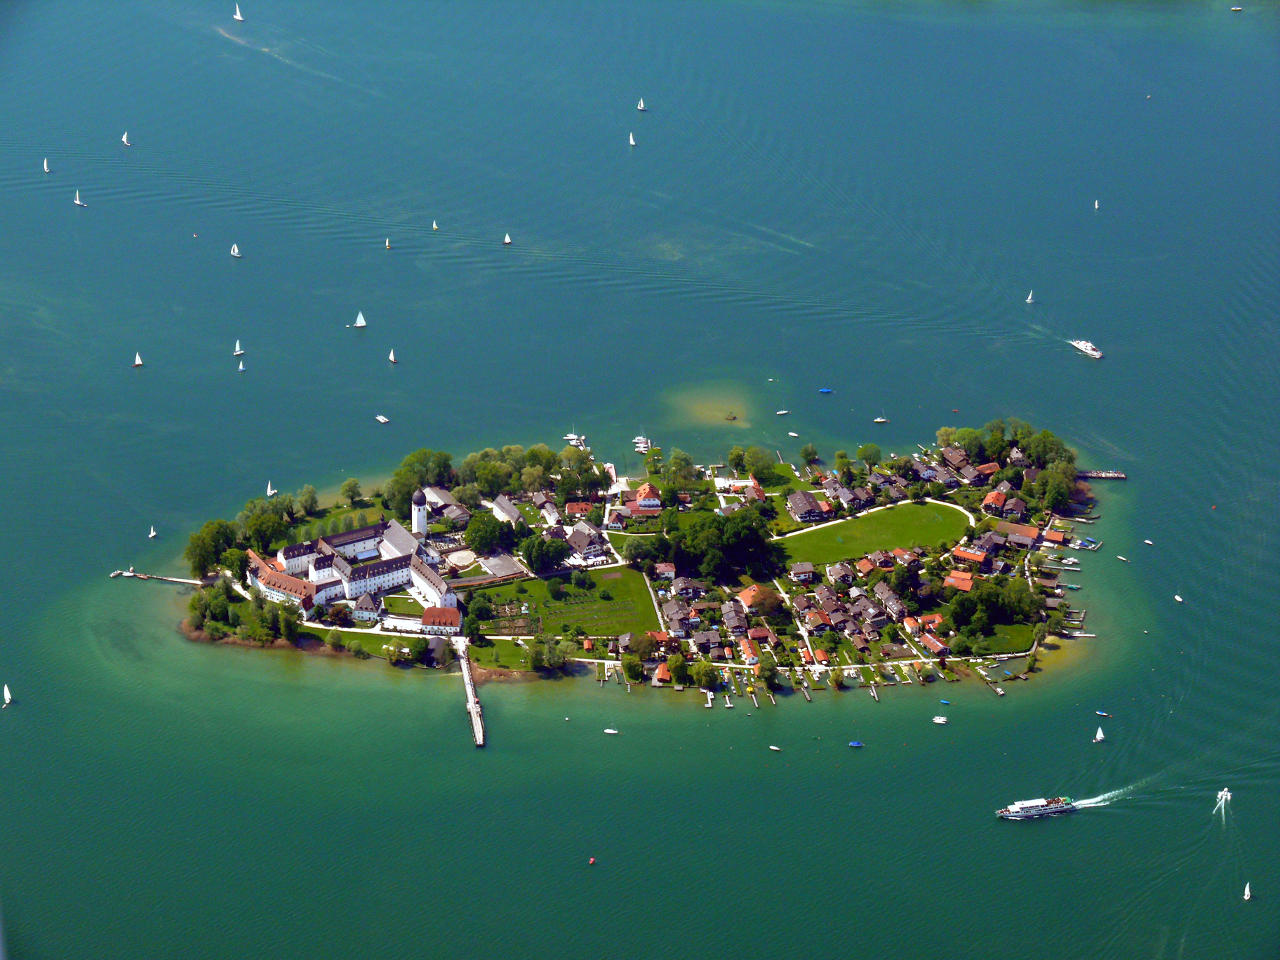
\includegraphics[height=\paperheight]{Chiemsee_Fraueninsel_scaled.JPG}
        };
    \end{tikzpicture}
\end{frame}

\againframe<2->{timeplace}

\begin{frame}
\frametitle{Grading}
  \begin{tabular}{lrl}
             & \alert{40 \%}   & Final Paper (Content, Style, Language, Scope, \ldots)\\
	     & \alert{10 \%}   & Practical application (depends on topic)  \\
             & \alert{10 \%}   & Review      \\
             & \alert{30 \%}   & Presentation (Content, Style, Timeliness, \ldots) \\
             & \alert{10 \%}   & Discussion                                                   \\
    \midrule
	$\Sigma$ & \alert{100 \%}  & Total                                                        \\
  \end{tabular}
\end{frame}

\begin{frame}
	\begin{center}
		{\huge Questions?}

		\vspace{2cm}

		\begin{center}
			Contact us at \\ \texttt{peuckert@sec.in.tum.de, \\ tschirschnitz@sec.in.tum.de}
		\end{center}

		\vspace{1cm}

		\tiny
		\begin{center}
			\url{https://www.sec.in.tum.de/i20/teaching/common-flaws-in-protocolsecurity}
		\end{center}
	\end{center}
\end{frame}


\end{document}
